%%%%%%%%%%%%%%%%%%%%%%%%%%%%%%%%%%%%%%%%%%%%%%%%%%%%%%%%%%%%%%%%%%%%%
% LaTeX Template: Project Titlepage Modified (v 0.1) by rcx
%
% Original Source: http://www.howtotex.com
% Date: February 2014
% 
% This is a title page template which be used for articles & reports.
% 
% This is the modified version of the original Latex template from
% aforementioned website.
% 
%%%%%%%%%%%%%%%%%%%%%%%%%%%%%%%%%%%%%%%%%%%%%%%%%%%%%%%%%%%%%%%%%%%%%%

\begin{filecontents*}{ref.bib}
@conference{evo:07:cec,
  booktitle={IEEE Congress on Evolutionary Computation},
  title={An evolutionary search heuristic for solving QAP formulation in facility layout design},
  author={Ramkumar, A.S. and Ponnambalam, S.G. and Jawahar, N.},
  isbn={978-1-4244-1339-3},
  pages={4005--4011},
  year={2007},
  publisher={IEEE},
  doi={10.1109/CEC.2007.4424993},
  keywords={search problems,combinatorial mathematics,evolutionary computation,facilities layout,quadratic programming},
  language={spanish},
  hyphenation={spanish}
}
@conference{sm:10:advcomp,
  booktitle={The Fourth International Conference on Advanced Engineering Computing and Applications in Sciences, ADVCOMP},
  title={New Simulated Annealing Algorithm for Quadratic Assignment Problem},
  author={Shojaee, Kambiz and Mollai, Nima and Hossein Seyedkashi, S. M. and Neshati, Mohammad Mohsen},
  isbn={978-1-61208-101-4},
  pages={87--92},
  year={2010},
  publisher={IARIA},
  % doi={10.1109/CEC.2007.4424993},
  keywords={search problems,combinatorial mathematics,simulated annealing,quadratic programming},
  language={spanish},
  hyphenation={spanish}
}

@book{koopmans1957assignment,
  title={Assignment Problems and the Location of Economic Activities},
  author={Koopmans, T.C. and Beckmann, M.J.},
  series={Bobbs-Merrill reprint series in economics},
  url={https://books.google.es/books?id=Kjs24p57FxgC},
  year={1957},
  publisher={Cowles Foundation for Research in Economics at Yale University}
}

@book{aarts1989simulated,
  title={Simulated annealing and Boltzmann machines: a stochastic approach to combinatorial optimization and neural computing},
  author={Aarts, E.H.L. and Korst, J.},
  isbn={9780471921462},
  lccn={88020871},
  series={Wiley-Interscience series in discrete mathematics and optimization},
  url={https://books.google.es/books?id=K\_pQAAAAMAAJ},
  year={1989},
  publisher={Wiley}
}

@misc{web:qaplib,
  title={QAPLIB - A Quadratic Assignment Problem Library},
  author={Burkard, R.E. and Çela, E. and Karisch, S.E. and Rendl, F.},
  month={06},
  year={2018},
  url={http://anjos.mgi.polymtl.ca/qaplib/}
}
\end{filecontents*}

\documentclass[12pt]{report}
\usepackage[a4paper]{geometry}
\usepackage[myheadings]{fullpage}
\usepackage{fancyhdr}
\usepackage{lastpage}
\usepackage{graphicx, wrapfig, subcaption, setspace, booktabs, epstopdf}
\usepackage[T1]{fontenc}
\usepackage[utf8]{inputenc}
\usepackage[font=small, labelfont=bf]{caption}
\usepackage{fourier}
\usepackage[protrusion=true, expansion=true]{microtype}
\usepackage[spanish]{babel}
\usepackage{sectsty}
\usepackage{url, lipsum}
\usepackage{amsmath}
\usepackage{listings}
\usepackage{color}

\usepackage{mathtools}
\DeclarePairedDelimiter\ceil{\lceil}{\rceil}
\DeclarePairedDelimiter\floor{\lfloor}{\rfloor}

\epstopdfsetup{update}
\DeclareGraphicsExtensions{.ps}
\epstopdfDeclareGraphicsRule{.ps}{pdf}{.pdf}{ps2pdf -dEPSCrop -dNOSAFER #1 \OutputFile}

\usepackage[bibencoding=auto,backend=biber,autolang=other]{biblatex}
\usepackage{csquotes}
\addbibresource{ref.bib}
\fancypagestyle{bibfooter}{\fancyhf{}\renewcommand{\headrulewidth}{0pt}\fancyfoot[R]{Fin}}

\renewcommand{\lstlistingname}{Código}
\renewcommand{\lstlistlistingname}{Lista de \lstlistingname s}

\definecolor{pblue}{rgb}{0.13,0.13,1}
\definecolor{pgreen}{rgb}{0,0.5,0}
\definecolor{pred}{rgb}{0.9,0,0}
\definecolor{pgrey}{rgb}{0.46,0.45,0.48}

\newcommand{\HRule}[1]{\rule{\linewidth}{#1}}
\onehalfspacing
\setcounter{tocdepth}{5}
\setcounter{secnumdepth}{5}

%-------------------------------------------------------------------------------
% LISTING CONFIG
%-------------------------------------------------------------------------------

\lstset {
    commentstyle=\color{pgreen},
    showstringspaces=false,
    keywordstyle=\color{pblue},
    stringstyle=\color{pred},
    basicstyle=\footnotesize\ttfamily,
    rulecolor=\color{black}
}

%-------------------------------------------------------------------------------
% HEADER & FOOTER
%-------------------------------------------------------------------------------
\pagestyle{fancy}
\fancyhf{}
\setlength\headheight{15pt}
\fancyhead[L]{\S\ David Lilue}
\fancyhead[R]{Universidad Politécnica de Madrid}
\fancyfoot[R]{Pag. \thepage\ de \pageref{LastPage}}
%-------------------------------------------------------------------------------
% TITLE PAGE
%-------------------------------------------------------------------------------

\usepackage[ddmmyyyy]{datetime}
\newdateformat{mydate}{Junio, \THEYEAR}

\begin{document}

\title{ \normalsize \textsc{Análisis y Procesado de Datos e Información - Computación Numérica Avanzada}
        \\ [2.0cm]
        \HRule{0.5pt} \\
        \LARGE \textbf{\uppercase{Análisis e implementación de distintas meta-heurísticas para el problema de la asignación cuadrática (QAP)}}
        \HRule{2pt} \\ [0.5cm]
        \normalsize \mydate\today \vspace*{3\baselineskip}\\
        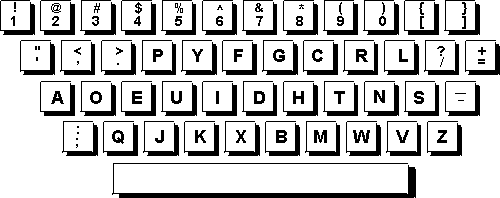
\includegraphics[scale=.45]{dvorak.png}\vfill}

\date{}

\author{
        David Lilue Borrero \\
        Universidad Politécnica de Madrid \\
        Departamento de Lenguajes y Sistemas Informáticos e\\ Ingeniería de Softwares }

\maketitle
\tableofcontents
\thispagestyle{empty}
\newpage

%-------------------------------------------------------------------------------
% Section title formatting
\sectionfont{\scshape}
%-------------------------------------------------------------------------------

%-------------------------------------------------------------------------------
% BODY
%-------------------------------------------------------------------------------

\section*{Introducción}
\addcontentsline{toc}{section}{Introducción}

En este trabajo tiene como objetivo general describir, analizar y probar distintas heurísticas para resolver el problema de la asignación cuadrática (QAP). Este problema tiene muchas aplicaciones en la vida real y es uno de los problema fundamentales de optimización combinatoria. Una motivación para escoger este problema es su complejidad, dado que involucra dos variables a la solución; como su nombre lo dice. Sus aplicaciones van desde el posicionamiento de componentes electrónicos en una placa hasta la distribución de letras en un teclado, buscando la eficiencia y minimización de costos. 

En específico se han trabajado como algoritmos de búsqueda local como un primer acercamiento al problema, estos tienden a tener un buen desempeño, pueden ajustarse e incorporarse a otras heurísticas; y así tener un mejor rendimiento para el proceso de optimización. En las próximas secciones se describe el problema, decisiones de implementación y casos de prueba para comprobar la eficacia del algoritmo.

Hay una sección dedicada a los algoritmos de búsqueda local que se usaron, para cada uno se hicieron distintas pruebas y se ajustaron para tener el mejor rendimiento, buscando comprobar e implementar los conceptos teóricos que describen cada algoritmo. Estos algoritmos posteriormente serán usados para complementar un algoritmo evolutivo, el cual permite la diversidad de soluciones dado por la naturaleza que lo inspiró. Al final se muestran distintos resultados de manera gráfica y así poder concluir las capacidades de cada algoritmo.

\newpage

\section*{Descripción del problema}
\addcontentsline{toc}{section}{Descripción del problema}

\selectlanguage{spanish}
El problema de la asignanción cuadratica, \textit{QAP} por sus siglas en inglés, es uno de los distintos problemas de optimización combinatoria que existen, por no decir uno de los más fundamentales y desafiantes de su clase. El mismo se puede explicar con un ejemplo de la vida real y que se usa a lo largo del desarrollo de este trabajo.

Partiendo de un conjunto de \textit{n} instalaciones y otro con \textit{n} localidades, para cada par de instalaciones existe una flujo y cada par de localidades una distancias. El objetivo es diseñar un plano de las instalaciones, asignándolas a distintas localidades y minimizando la suma de las distancias por el respectivo flujo. Esto se puede ver en compañías de manufactura, dado que puede implicar mayor costo y ineficiencia en sus operaciones\cite{evo:07:cec}.

Se puede enunciar formalmente usando dos matrices de dimensiones $n\times n$, denominadas $D = (d_{ij})$ y $F = (f_{ij})$, la distancia entre dos localidades y el flujo entre dos instalaciones respectivamente. La idea es encontrar la permutación $\Pi$ de las instalaciones asignadas que minimice la siguiente suma\cite{sm:10:advcomp}.

\[\substack{\text{\large min} \\ \pi}\sum_{ij}^{n} d_{ij}f_{\pi(i)\pi(j)}\]

\subsection*{Lenguaje de programción}
\addcontentsline{toc}{subsection}{Lenguaje de programción}

Para realizar el trabajo se ha usado \texttt{Python} como lenguaje de programación, la razón de esta decisión viene dada porque el mismo provee un nivel de abstracción con un sistema orientado a objetos y a su vez permite tener ejecuciones con tiempo relativamente eficientes. Además de reducir el tiempo de implementación en comparación a otros lenguajes que pueden tener mayor desempeño computacional, como son \texttt{C} o \texttt{C++}, pero resulta difícil de implementar una solución en un tiempo aceptable y con uso eficiente de memoria.

\subsection*{Esturcturas y representación}
\addcontentsline{toc}{subsection}{Esturcturas y representación}

La representación del problema y sobretodo de una solución usan \texttt{numpy}, una librería para manejar datos numéricos en colecciones como arreglos o matrices, para mantener la información de las distancias entre localidades como una matriz de adyacencia donde cero ($0$) implica que no hay comunicación entre ellas, sino se especifica la distancia. También se mantiene una matriz con el flujo entre las instalaciones, de manera similar a la representación de las distancias.

Toda esta información es almacenada como atributos de una clase, logrando encapsular el comportamiento de una solución de forma abstracta. Es de esperar que existen otros atributos como el valor de la función objetivo aplicada a la solución y otro con la permutación de las instalaciones, estos atributos son los propiedades que nos permitirán comparar distintas soluciones e ir minimizando la misma. La clase utilizada es la que se muestra a continuación, sin mostrar distintos métodos que la misma tiene implementados.

\begin{lstlisting}[language=Python]
        import numpy as np
         
        class Solution:
            def __init__(self, n, ds, fs):
                self.n = n
                self.permutation = np.array(xrange(1,n+1))
                self.distances = np.array(ds)
                self.flows = np.array(fs)
                self._cost = None
\end{lstlisting}

\subsection*{Instancias del problema}
\addcontentsline{toc}{subsection}{Instancias del problema}

Para probar el desempeño y proximidad a soluciones óptimas de los diferentes algoritmos se utiliza un conjunto de instancias y soluciones usadas en distintos artículos y autores que se listan en el portal web de \texttt{QAPLIB}\cite{web:qaplib}. Para este trabajo se usan cuatro instancias con distintas dimensiones y cantidad de flujo entre las instalaciones. Cada una es pasada como entrada a los distintos algoritmos y se intenta ajustar los parámetros para hacer la mayor cantidad de pruebas. Dejando la posibilidad de llegar una conclusión amplia.

Este \textit{dataset} se ha ajustado a un mismo formato para generalizar la lectura de los archivos desde el \textit{script}. Es importante destacar que las matrices escogidas son simétricas y la diagonal principal presenta solamente ceros. Esto se debe a que los casos aplican a la vida real donde las localidades no tiene distancia entre ellas mismas y entre una misma instalación no hay flujo. A continuación se muestra un ejemplo de como sería un archivo de entrada.

\begin{lstlisting}
        5

        0  1  2  3  1
        1  0  1  2  2
        2  1  0  1  3
        3  2  1  0  4
        1  2  3  4  0
\end{lstlisting}

\newpage

\begin{lstlisting}
        0  5  2  4  1
        5  0  3  0  2
        2  3  0  0  0
        4  0  0  0  5
        1  2  0  5  0
\end{lstlisting}

Comenzando con la dimensión de las matrices, ambas cuadradas, siguiendo la matriz de distancias y de segunda la de flujos.

\section*{Búsqueda local}
\addcontentsline{toc}{section}{Búsqueda local}

Comenzando con un algoritmo simple de búsqueda local que son ampliamente usados para resolver problemas de optimización. La implementación que se muestra a continuación altera aleatoriamente una solución (intercambiando instalaciones en distintas localidades) tantas veces con indique un coeficiente que va relacionado con la dimensión de la solución y en caso de conseguir una permutación mejor, esta perdura a la próxima iteración. Sino se regresa a la solución que hasta el momento es la que tiene mínimo costo.

\begin{lstlisting}[language=Python]
    def search(sln, iterations_coeff=LOCAL_SEARCH_COEFFICIENT):
        for _ in xrange(0, int(iterations_coeff * sln.n)):
            cities = randomOptions(sln.n, k=2)
            aux_cost = sln.cost
    
            sln.exchangeFacilities(cities[0], cities[1])
    
            if aux_cost < sln.cost:
                sln.exchangeFacilities(cities[0], cities[1])
    
        return sln
\end{lstlisting}

A continuación se presenta una gráfica comparativa del algoritmo al incrementar el coeficiente de iteración, en específico a una instancia de dimensión 12, haciendo 100 corridas y comenzando con una permutación aleatoria. Usando un coeficiente de iteración mayor es de esperar que el tiempo de ejecución incrementará pero en todos los casos esta no supera una décima segundo.

\begin{center}
    \includegraphics[width=0.8\linewidth,height=\textheight,keepaspectratio]{nug12_ls.ps}
\end{center}

Como se puede observar, el desempeño tiende a mejorar al incrementar el número de iteraciones pero este comportamiento es asintótico. Llegando en algunos casos a conseguir la solución óptima, resaltada con la linea roja. Esto nos ayuda a conseguir la mejor configuración de los parámetros para el algoritmo, que más adelante se usa con un algoritmo evolutivo.

El principal inconveniente con este algoritmo es que tiende a quedarse en mínimos locales porque la perturbación es leve por ello se ha implementado el algoritmo de \textit{simulated annealing} que se enuncia en la próxima sección.

\subsection*{Simulated annealing}
\addcontentsline{toc}{subsection}{Simulated annealing}

Este algoritmo fue propuesto por Koopsmans y Beckmann en 1957\cite{koopmans1957assignment}, posteriormente se aplicó a QAP. Está basado en un proceso usado en metalurgia para alterar las propiedad físicas y químicas de distintos metales. Inspirando un algoritmo que tiene un factor de energía o temperatura, que indica la probabilidad de aceptar soluciones que pueden no ser mejores a la actual pero permite tener una búsqueda más global en el espacio de soluciones\cite{sm:10:advcomp}.

La estrategia de enfriamiento es uno de los elementos fundamentales para que el algoritmo se comporte como se espera y encuentre una buena solución, de igual manera la temperatura inicial juega un papel importante para que esta energía mueva la solución en el espacio.

\newpage

\begin{lstlisting}[language=Python]
    def annealing(sln, t_max=ANNEALING_TEMPERATURE_MAX):
        t = t_max
        k = 0.0
    
        while t > 0.0:
            aux_sln = sln.copy()
            aux_sln.randomize(sln.n if t > sln.n else int(t))
    
            diff_cost = sln.cost - aux_sln.cost
    
            if diff_cost > 0 or \
               math.exp(float(diff_cost) / t) > random.uniform(0,1):
                sln.permutation = aux_sln.permutation
                sln.flows = aux_sln.flows
                sln.cost = aux_sln.cost
    
            del aux_sln
            k += 1.0
            t = math.floor(t_max / (1.0 + MULT_FAC * math.log10(1+k)))
\end{lstlisting}

La temperatura inicial o máxima desde la que parte el algoritmo es proporcional a la alteración que sufre la solución, por lo que su búsqueda es más global mientras la temperatura sea grande pero eso conlleva a un número mayor de iteraciones. Entonces es complicado encontrar la configuración inicial que se adapte al problema.

La función utilizada como estrategia de enfriamiento está fundamentada en un comportamiento logarítmico\cite{aarts1989simulated}, esto permite tener valores altos para iteraciones más jóvenes y a lo largo de la ejecución va ir disminuyendo lentamente a 0. La definición formal de la función se puede ver a continuación.

\[T_{k+1} = \floor*{ \frac{T_0}{1 + \alpha\times\log_{10} (1 + k) }}\ ,\ \alpha > 1\]

A continuación se puede ver como se comporta el algoritmo a distintas temperaturas. El tiempo de ejecución es mayor al algoritmo de la sección anterior pero no excede el segundo y medio.
 
\begin{center}
    \includegraphics[width=0.9\linewidth,height=\textheight,keepaspectratio]{nug12_sa.ps}
\end{center}

\subsection*{Búsqueda local iterativa}
\addcontentsline{toc}{subsection}{Búsqueda local iterativa}

Tratando de mejorar un poco la búsqueda local que se vio antes, se implementa una iterativa que sea más ambiciosa, intentando de salir de los mínimos locales y así llegar al óptimo. Manteniendo similitud con el primer algoritmo, este incorpora mayor alteración (factor de mutación) a la solución actual mientras no se encuentra alguna mejor hasta que encuentre alguna y se aplica una recompensa en caso de encontrar una con menor costo.

Generalmente este tipo de algoritmos tiene un mejor desempeño pero el tiempo de ejecución es mayor, el objetivo es tener una ganancia considerable sin perder la eficiencia. Incorporando un factor de mutación (relación de la cercanía al final de la ejecución) permite tener una vista más amplia de la vecindad a partir de una solución, y una ventaja es que esta exploración es progresiva. A diferencia de \textit{simulated annealing}, que inicia con gran aleatoriedad y finaliza siendo más recatado.

\newpage

\begin{lstlisting}[language=Python]
  def eager_search(sln, iterations_coeff=LOCAL_SEARCH_COEFFICIENT):
      crnt_it = 0.0
      max_it_f = iterations_coeff * sln.n

      while crnt_it < max_it_f:
          crnt_it += 1.0
          mutation_factor = crnt_it / max_it_f
          aux_sln = sln.copy()

          for i in xrange(0, int(math.ceil(mutation_factor * sln.n))):
              aux_sln.randomize()
              
              if aux_sln.cost < sln.cost:
                  sln.permutation = aux_sln.permutation
                  sln.flows = aux_sln.flows
                  sln.cost = aux_sln.cost
                  crnt_it = 0
                  break
          del aux_sln
      return sln
\end{lstlisting}

Como puede verse a continuación, el desempeño es mejor al momento de encontrar la solución óptima pero tener un coeficiente grande implica que las soluciones comienzan a dispersarse más. Dado que este guarda relación con el factor de mutación y eso puede tener ventajas como desventajas.

\begin{center}
    \includegraphics[width=0.78\linewidth,height=\textheight,keepaspectratio]{nug12_ils.ps}
\end{center}

\newpage

En los siguientes gráficos se puede ver como se comportan los algoritmos lado a lado con una instancia de dimensiones $n=19$, que tanto se aproximan a la solución óptima y el tiempo de ejecución.

\begin{figure}[h]
    \centering
    \begin{minipage}{0.5\textwidth}
        \centering
        \includegraphics[width=0.95\textwidth]{els19_all.ps} % first figure itself
        % \caption{first figure}
    \end{minipage}\hfill
    \begin{minipage}{0.5\textwidth}
        \centering
        \includegraphics[width=0.95\textwidth]{els19_t_all.ps} % second figure itself
        % \caption{second figure}
    \end{minipage}
\end{figure}

\section*{Algoritmo evolutivo}
\addcontentsline{toc}{section}{Algoritmo evolutivo}

Los algoritmos evolutivos han sido usado en muchos áreas de la optimización combinatoria\cite{evo:07:cec} y en este trabajo se combina con los algoritmos de búsqueda local que se presentaron anteriormente para tener un enfoque más amplio del problema que se está analizando.

Con la ayuda de este tipo de algoritmos se busca la diversidad de soluciones, basándose en un concepto de la evolución en biología. Partiendo de una población inicial, realizando procesos de reproducción y mutación en las distintas generaciones con el objetivo de tener diversidad y escoger a los mejores candidatos para reproducir en cada generación.

En nuestro caso se ha escogido una población aleatoria inicial de 60 soluciones y se reproducir durante 7 generaciones. Cada par de padres tendrá 3 hijos, a estos se les aplicará una búsqueda local y serán descartados aquellos que tengan las peores cualidades. La idea es ver como se comporta el algoritmo evolutivo con las distintas búsquedas locales con diferentes instancias.

A continuación se puede ver como se comporta el algoritmo genético dependiendo de que búsqueda local se utilice.

\newpage

\section*{Conclusiones}
\addcontentsline{toc}{section}{Conclusiones}
\lipsum[1]

%-------------------------------------------------------------------------------
% REFERENCES
%-------------------------------------------------------------------------------
\newpage

\printbibliography
\thispagestyle{bibfooter}

\end{document}

%-------------------------------------------------------------------------------
% SNIPPETS
%-------------------------------------------------------------------------------

%\begin{figure}[!ht]
%   \centering
%   \includegraphics[width=0.8\textwidth]{file_name}
%   \caption{}
%   \centering
%   \label{label:file_name}
%\end{figure}

%\begin{figure}[!ht]
%   \centering
%   \includegraphics[width=0.8\textwidth]{graph}
%   \caption{Blood pressure ranges and associated level of hypertension (American Heart Association, 2013).}
%   \centering
%   \label{label:graph}
%\end{figure}

%\begin{wrapfigure}{r}{0.30\textwidth}
%   \vspace{-40pt}
%   \begin{center}
%       \includegraphics[width=0.29\textwidth]{file_name}
%   \end{center}
%   \vspace{-20pt}
%   \caption{}
%   \label{label:file_name}
%\end{wrapfigure}

%\begin{wrapfigure}{r}{0.45\textwidth}
%   \begin{center}
%       \includegraphics[width=0.29\textwidth]{manometer}
%   \end{center}
%   \caption{Aneroid sphygmomanometer with stethoscope (Medicalexpo, 2012).}
%   \label{label:manometer}
%\end{wrapfigure}

%\begin{table}[!ht]\footnotesize
%   \centering
%   \begin{tabular}{cccccc}
%   \toprule
%   \multicolumn{2}{c} {Pearson's correlation test} & \multicolumn{4}{c} {Independent t-test} \\
%   \midrule    
%   \multicolumn{2}{c} {Gender} & \multicolumn{2}{c} {Activity level} & \multicolumn{2}{c} {Gender} \\
%   \midrule
%   Males & Females & 1st level & 6th level & Males & Females \\
%   \midrule
%   \multicolumn{2}{c} {BMI vs. SP} & \multicolumn{2}{c} {Systolic pressure} & \multicolumn{2}{c} {Systolic Pressure} \\
%   \multicolumn{2}{c} {BMI vs. DP} & \multicolumn{2}{c} {Diastolic pressure} & \multicolumn{2}{c} {Diastolic pressure} \\
%   \multicolumn{2}{c} {BMI vs. MAP} & \multicolumn{2}{c} {MAP} & \multicolumn{2}{c} {MAP} \\
%   \multicolumn{2}{c} {W:H ratio vs. SP} & \multicolumn{2}{c} {BMI} & \multicolumn{2}{c} {BMI} \\
%   \multicolumn{2}{c} {W:H ratio vs. DP} & \multicolumn{2}{c} {W:H ratio} & \multicolumn{2}{c} {W:H ratio} \\
%   \multicolumn{2}{c} {W:H ratio vs. MAP} & \multicolumn{2}{c} {\% Body fat} & \multicolumn{2}{c} {\% Body fat} \\
%   \multicolumn{2}{c} {} & \multicolumn{2}{c} {Height} & \multicolumn{2}{c} {Height} \\
%   \multicolumn{2}{c} {} & \multicolumn{2}{c} {Weight} & \multicolumn{2}{c} {Weight} \\
%   \multicolumn{2}{c} {} & \multicolumn{2}{c} {Heart rate} & \multicolumn{2}{c} {Heart rate} \\
%   \bottomrule
%   \end{tabular}
%   \caption{Parameters that were analysed and related statistical test performed for current study. BMI - body mass index; SP - systolic pressure; DP - diastolic pressure; MAP - mean arterial pressure; W:H ratio - waist to hip ratio.}
%   \label{label:tests}
%\end{table}
